\documentclass[10pt,conference,a4paper]{IEEEtran}
\usepackage[utf8]{inputenc}
\usepackage[T1]{fontenc}
% Correct date format in references but with american hyphenation, quotes, ...
% Trick from http://tex.stackexchange.com/a/129209
\usepackage[australian,american]{babel}

% *** GRAPHICS RELATED PACKAGES ***
\ifCLASSINFOpdf
  \usepackage[pdftex]{graphicx}
\else
  \usepackage[dvips]{graphicx}
\fi

% *** MATH PACKAGES ***
\usepackage{amssymb}
\usepackage[cmex10]{amsmath}

% Figure captions in small font
\makeatletter
\let\MYcaption\@makecaption
\makeatother
\usepackage[font=footnotesize]{subcaption}
\makeatletter
\let\@makecaption\MYcaption
\makeatother

\usepackage{pgfplots}
\pgfplotsset{compat=1.9}
%TODO minted ?
\usepackage[binary-units]{siunitx}
\usepackage{booktabs}
\usepackage{pifont}
\usepackage{tikz}
\usepackage{csquotes}
\usepackage[backend=biber,style=ieee,minbibnames=1,maxbibnames=3]{biblatex}
\usepackage{url}
\usepackage[backgroundcolor=lightgray]{todonotes}
\usepackage[hidelinks]{hyperref}


\bibliography{paper}
% Small font for references
\renewcommand*{\bibfont}{\small}

% correct bad hyphenation here
\hyphenation{op-tical net-works semi-conduc-tor}

% paper title
% can use linebreaks \\ within to get better formatting as desired
\def\mytitle{EpTO: An Epidemic Total Order Algorithm for Large-Scale Distributed Systems}
\title{\mytitle}

% author names and affiliations
% use a multiple column layout for up to three different
% affiliations
\def\jocelyn{Jocelyn Thode}
\def\ehsan{Ehsan Farhadi}
\author{
	\IEEEauthorblockN{\jocelyn}
	\IEEEauthorblockA{Université de Fribourg\\
	Fribourg, Switzerland\\
	Email:\href{mailto:jocelyn.thode@unifr.ch}{jocelyn.thode@unifr.ch}
	}
	\and
	\IEEEauthorblockN{\ehsan}
	\IEEEauthorblockA{Université de Neuchâtel\\
		Neuchâtel, Switzerland\\
		Email:\href{mailto:ehsan.farhadi@unine.ch}{ehsan.farhadi@unine.ch}
	}
	
}

% Set PDF file properties
\hypersetup{
	pdftitle=\mytitle,
}

% Tick marks
\newcommand{\cmark}{\ding{51}}
\newcommand{\xmark}{\ding{55}}

% Columns balancing
\renewbibmacro{finentry}{%
  \iffieldequalstr{entrykey}{jujjuri2010virtfs}%<- key after which you want the break
   {\finentry\newpage}
   {\finentry}}

\begin{document}
\graphicspath{{figures/}}


% make the title area
\maketitle


\begin{abstract}
Total ordering has always been of interest in large-scale distributed systems. EpTO is one of the recently introduced total order algorithms for large-scale distributed systems and claims to provide total order and scalability at the same time. In this paper, we verify this claim by implementing EpTO and evaluate its reliability in real-world conditions. We then compare it to a deterministic total order algorithm named JGroups.
\end{abstract}
\section{Introduction}
Creating an algorithm providing scalability, integrity and validity, along with a total ordering for the events through all peers in a distributed system has been one the hot topics in distributed systems research for many years. One of the recently designed algorithms on this topic is EpTO \autocite{matos2015epto}. EpTO is an algorithm which claims to provide integrity, validity and total order in a large-scale distributed system. In addition, EpTO is designed to work without a global clock, thus is well-suited for dynamic large-scale distributed systems.
\par 
There are many other algorithms for disseminating and ordering events in a distributed system. There are some deterministic algorithms, which guarantee total order, agreement or other strong properties. Unfortunately, these types of algorithm are not scalable enough to be used in a large-scale distributed system \autocites[]{defago2004total}[]{lamport1978time}.
\par
The problem with existing deterministic total ordering protocols is that they need some sort of agreement between all peers in the system. This causes a massive amount of network traffic and overhead on the system.
Moreover, an agreement feature for an asynchronous system requires to
explicitly maintain a group and have access to a failure detector \autocites[]{chandra1996weakest}[]{chandra1996unreliable}. Due to faults and churn in large-scale distributed systems, failure detector turns into a bottleneck for the system and thus, limits the scalability of the algorithm.
\par
As an alternative to deterministic algorithms, there are probabilistic algorithms, focusing on scalability and resiliency against failures using a probabilistic dissemination approach \autocites []{birman1999bimodal}[]{carvalho2007emergent}[]{demers1987epidemic}[]{eugster2003lightweight}[]{felber2002probabilistic}[]{hayden1996probabilistic}[]{kim2004gossip}[]{Koldehofe02simplegossiping}. These algorithms guarantee the dissemination of events in the system with high probability. This way, there is no need for failure detectors and redundant traffic, making these algorithms highly scalable. Although as these algorithms focus on reliability of dissemination, they often have to ignore other properties such as total ordering.
\par
This is where EpTO comes into light. EpTO, by mixing these two types of algorithms, provides total order along with scalability, validity and integrity. 
EpTO consists of two distinct parts. The first part is probabilistic dissemination. EpTO guarantees that all peers will receive an event with arbitrarily high probability. The second part of EpTO is deterministic ordering. Once peers have received all events, they will deterministically order them using the events timestamp, and in case of a tie use the event's broadcaster id.
\par
To model the first part, EpTO is using a \textit{balls-and-bins} approach \autocite{Koldehofe02simplegossiping}. The balls-and-bins problem is a basic probabilistic problem: consider \textit{n} balls and \textit{m} bins where we consequently throw balls into a bin completely random and independent from other balls. In this scenario, one of the natural questions that comes to mind is: what is the minimum number of balls that should be thrown, so that every bin has at least one ball?
\begin{figure}
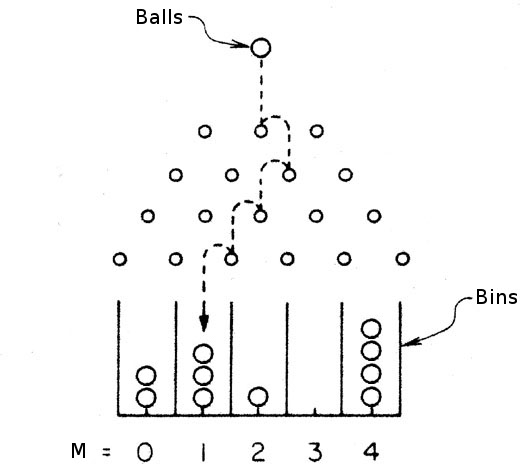
\includegraphics[width=\linewidth]{figures/BnB.jpeg}
\caption{Balls-and-Bins}
\label{fig:balls-and-bins}
\end{figure}
\par
Using the balls-and-bins approach we model processes as bins and events as balls. Based on this model we will calculate how many balls need to be \textit{thrown} such that every bin contains at least one ball with arbitrarily high probability. Using this approach the number of messages transmitted per process per round is logarithmic in the number of processes, therefore the number of messages sent in the system is low and uniform over all processes. Using these approaches, EpTO becomes highly scalable and resilient, while still providing total order.

\subsection{Contribution}
Until now, the creators of EpTO have only tested this algorithm in a simulated environment. In this work, We are going to implement EpTO in pure Java using the NeEM library \autocite{neem} and show that EpTO is actually suitable for real-world large-scale distributed systems. We then evaluate EpTO by comparing it to the deterministic total order algorithm provided by JGroups  \autocite{jgroups} in both stable (no-churn) and unstable systems. These comparisons help us verify if EpTO is actually performing as expected in a real-world scenario.
\todo[inline]{Here we present our conclusion briefly}
\par
These tasks are split in two parts. The first part will assume that all peers are known by all peers. We will implement EpTO using this assumption and test it against JGroups. In the second part of the tasks, we will assume unknown membership on all peers. We will update EpTO and use a PSS\footnote{Peer Sampling Service} to find peers to exchange with. We will then update the underlying layer NeEM to use UDP instead of TCP and switch to NIO.2 \todo{NIO2?} \autocite{nio}.

\section{Ordering Algorithms}
Distributed systems, like centralized systems, need to preserve the temporal order of events produced by concurrent processes in the system. When there are separated processes that can only communicate through messages, you can’t easily order these messages.
Therefore we need ordering algorithms to overcome this problem.
\par
We have two types of ordering algorithms \autocite{lamport1978time}: the partial order algorithms and the total order algorithms.
\subsection{Partial Order Algorithms}
Assuming S is partially ordered under $\leq$, then the following statements hold for all a, b and c in S:
\begin{itemize}
	\item Reflexivity: $a \leq a$ for all $a \in S$.
	\item Antisymmetry: $a \leq b$ and $b \leq a$ implies $a=b$ .
	\item Transitivity: $a \leq b$  and $b \leq c$  implies $a \leq c$.
\end{itemize}

\subsection{Total Order Algorithms}
A totally ordered set of events is a partially ordered set which satisfies one additional property:
\begin{itemize}
	\item Totality (trichotomy law): For any $a, b \in S$, either $a \leq b$  or $b \leq a$.
\end{itemize}
\par
In other words, total order is an ordering that defines the exact order of every event in the system. On the other hand, partial ordering only defines the order between certain key events that depend on each other. Partial order can be useful since it is less costly to implement. However, in some cases the order of all events is important, for example when we need to know exactly which operations have been invoked in which order, we have to use total order, otherwise we could end up in an inconsistent state.

\section{EpTO}
\begin{figure}
	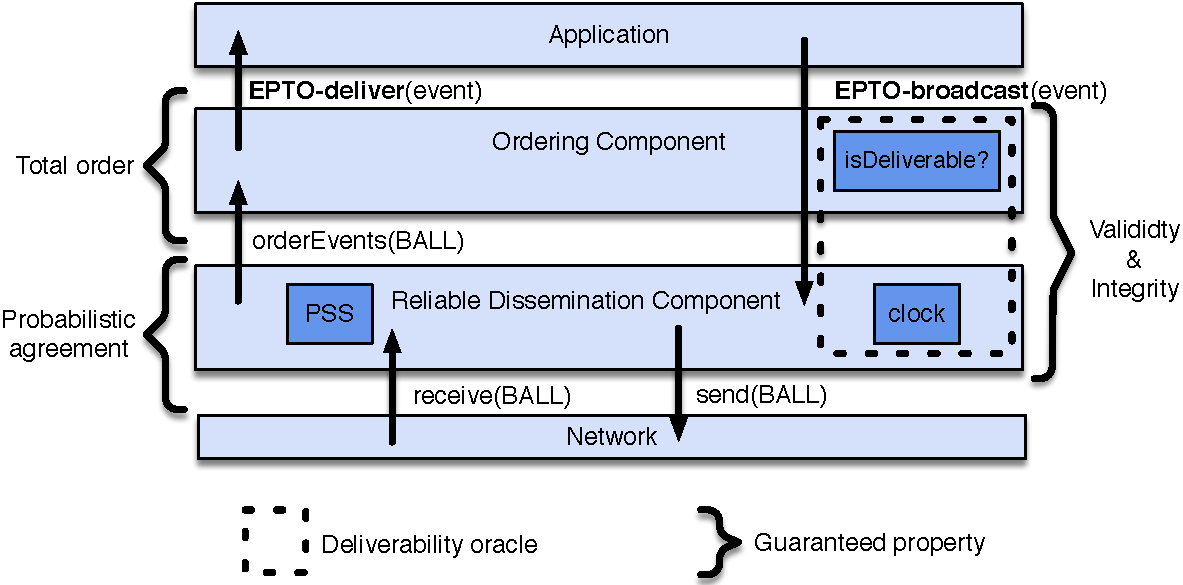
\includegraphics[width=\linewidth]{figures/architecture.pdf}
	\caption{EpTO architecture \autocite{matos2015epto}}
	\label{fig:epto-architecture}
\end{figure}
\subsection{Definitions}
A process or peer is defined as an actor in our system running the application that needs total order. Each process will communicate with other processes in the distributed systems and exchange events and order them together.
\par
An event is defined as something that happens at a given time. For example, we could imagine a system where each process publish some sort of data. The moment where this data is published combined with the data is called an event.
\par
A ball is a set of events bundled together and sent as one package. We use balls in EpTO to reduce network traffic and make it scalable in terms of processes and events.

We define scalable as it was defined in  \autocite{matos2015epto}:  ``The number
of messages transmitted per process per round is logarithmic
in the number of processes, ...''

\par
Since EpTO is using a probabilistic agreement instead of a deterministic agreement, there might be a situation where a peer does not receive an event (with a very low arbitrary probability). In this case there will be a hole in the sequence of delivered events but even in this case, the order of the delivered event will be protected by EpTO's deterministic ordering algorithm and total order property is preserved.
\subsection{Dissemination Component}
The Dissemination component is the component that bridges EpTO with the rest of the network. As we can see in  \todo{Hugues comment} Figure \ref*{fig:epto-architecture}, it is in charge of receiving balls it opens them, passes them to the Ordering component and then forwards them to \textit{K} other processes, where K denotes the gossip fan-out.
\par
When an application wants to publish an event, it will broadcast this event to the Dissemination component.

\subsection{Ordering Component}
The Ordering component is responsible for ordering events before delivering them to the application.
To achieve this, the Ordering component has a \textit{received} hash table of (\textit{id}, \textit{event}) pairs containing all the events which are received by the peer, but not yet delivered to the application and a \textit{delivered} hash table containing all the events which are delivered.
\par
In brief, the Ordering component first increments the timestamp of all the events which have been received in previous rounds to indicate the start of a new round. Then, it processes new events in the received ball by discarding events that have been received already (delivered events or events with timestamp smaller than the last delivered event). This is done to prevent delivering duplicate events. The remaining events in the received ball will be added to the \textit{received} hash table, and wait to be delivered based on the Stability oracle.
\subsection{Stability Oracle}
The Stability oracle is the component that outputs timestamps. It will increment its local clock every round as well as synchronize itself using timestamps of newly received events, to make sure the local clock does not drift too much.
\par
This Stability oracle offers an API to the Ordering component letting it know when an event is mature enough to be delivered to the application.
\par
As this component is local and only corrects itself when we receive new events, it generates no network traffic. This means it does not impact the scalability of EpTO.
\section{Performance Comparisons}
\todo[inline]{Here we will present the different test we ran, the methodology used and the result we obtained}
\subsection{Methodology}
\todo[inline]{Here we explain how we ran our tests and on what type of machines}
\subsection{Peer membership known}
\todo[inline]{We will present the results obtained and try to explain the results}
\subsection{Peer membership unknown}
\todo[inline]{We will present the results obtained and try to explain the results}

\section{Conclusion}
\todo[inline]{He we will summarize the results we found and present some future tasks that could be accomplished on EpTO}


% conference papers do not normally have an appendix


% use section* for acknowledgement
\section*{Acknowledgment}
\todo[inline]{Write acknowledgment}




% references section, with correct date format
\begin{otherlanguage}{australian}
\printbibliography
\end{otherlanguage}

% that's all folks
\end{document}
